\documentclass{article}
\usepackage{graphicx}
\usepackage[margin=1.5cm]{geometry}
\usepackage{amsmath}

\begin{document}

\title{Wednesday Reading Assessment: Unit 7, Power and Conservation of Energy}
\author{Prof. Jordan C. Hanson}

\maketitle

\section{Conservation of Energy}

\begin{enumerate}
\item A particle of mass m is hung from the ceiling by a massless string of length 1.0 m, as shown in Figure \ref{fig:pend}. The particle is released from rest, when the angle between the string and the downward vertical direction is 30 degrees.  What is its speed when it reaches the lowest point of its arc?
\begin{figure}[ht]
\centering
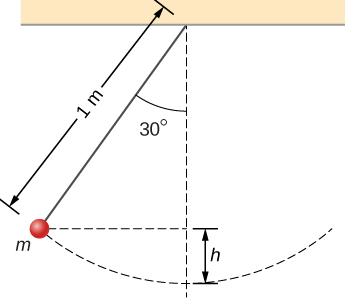
\includegraphics[width=0.4\textwidth]{pend.png}
\caption{\label{fig:pend} A particle hung from a string constitutes a simple pendulum. It is shown when released from rest, along with some distances used in analyzing the motion.}
\end{figure}
\item What is the gravitational potential energy as a function of the angle $\theta$? \\ \vspace{2cm}
\item Approximate the result in the prior question as some polynomial.
\end{enumerate}
\end{document}